% !TEX encoding = UTF-8 Unicode
% !TEX program = lualatex
%% !BIB program = bibtex
%        1         2         3         4         5         6         7  
%23456789012345678901234567890123456789012345678901234567890123456789012

\newif\ifforloop
\forlooptrue

\documentclass[12pt, aspectratio=169]{beamer}
    \parskip0pt
    \lineskip0pt
    \baselineskip0pt
    \setbeamertemplate{navigation symbols}{}
    \setbeamercolor{normal text}{fg=black}
	\setbeamercolor{structure}{fg=blue!80!black}
	\setbeamercolor{alerted text}{fg=red!70!black}
	\setbeamercolor{example text}{fg=green!60!black}
    \setbeamersize{text margin left=3mm,text margin right=3mm}
    \makeatletter
    \define@key{beamerframe}{c}{% true center
        \beamer@frametopskip=0pt plus 1fill\relax%
        \beamer@framebottomskip=0pt plus 1fill\relax%
    }
    \makeatother
    \setbeamertemplate{background canvas}{
        \begin{tikzpicture} [overlay, shift={(8, -4.5)}]
            \def\idep{\insertdocumentendpage}
            \pgfmathsetmacro\x {(\thepage - 1) / max(\idep - 1, 1)}
            \node at (10 * \x - 5, 0) [opacity=.2]
                {\includegraphics[width=26cm]{sfo.jpg}};
            \begin{scope}[line cap=butt, line join=butt,
                line width=16cm, dash pattern=on1cm off1cm]
                \draw [opacity=0.01, black] (-8, 0) -- (8, 0);
                \draw [opacity=0.1, white] (0, 5) -- (0, -5);
            \end{scope}
        \end{tikzpicture}
    }

\usepackage{mathtools, unicode-math, emoji}
    \setmainfont{NotoSans-Light}
    \setsansfont{NotoSans-Light}
    \setmonofont{NotoSans-Light}
    \setemojifont{Apple Color Emoji}
	\setmathfont{texgyrepagella-math.otf}

\usepackage{pst-barcode, tikz, tikz-cd, booktabs}
	\usetikzlibrary{arrows.meta}
    \usetikzlibrary{lindenmayersystems}
	\pgfmathdeclarefunction*{axis_height}{0}
		{\begingroup\pgfmathreturn.25em\endgroup}
	\pgfmathdeclarefunction*{rule_thickness}{0}
		{\begingroup\pgfmathreturn.06em\endgroup}
    \tikzset{
        every picture/.style
            = {cap=round, join=round, line width=rule_thickness},
        alt/.code args
            = {<#1>#2#3}{\alt<#1>{\pgfkeysalso{#2}}{\pgfkeysalso{#3}}},
        uncover/.style={alt=#1{}{opacity=.15}},
        only/.style={alt=#1{}{opacity=0}},
        %tex.stackexchange.com/q/146908
    }


                                 \title
              {Channel Manipulation as a Coding Technique}
                                    
                                \author
                             {Hsin-Po Wang}

                               \institute
                          {EECS, UC Berkeley}

\begin{document}

\centering

\begin{frame}
    \fontsize{40pt}{60pt}\selectfont
    \inserttitle
    
    \vskip1.5cm

    \fontsize{20pt}{0}\selectfont
    \insertauthor\qquad(\insertinstitute)
\end{frame}

\def\linkfil#1{\vbox to#1cm{\hbox{|}\vfil\hbox to3mm{\hfil|}}}
\defbeamertemplate*{sidebar left}{thinbold}{
	\pgfsetfillopacity0
	\hyperlinkframeendprev{\linkfil1}\vfil
	\hyperlinkslideprev{\linkfil3}\vfil
	\hyperlinkslidenext{\linkfil3}\vfil
	\hyperlinkframestartnext{\linkfil1}\vfilneg
	\pgfsetfillopacity1
}

\makeatletter
\defbeamertemplate*{sidebar right}{thinbold}{
	\begin{tikzpicture} [overlay, x=3mm, y=\paperheight]\scriptsize
		\pgfmathsetmacro\overlayfrac{\insertoverlaynumber/
            (\insertframeendpage+1-\insertframestartpage)}
		\path[save path=\P, yscale={1/max(\insertmainframenumber-1,1)}]
			(0,0)-|(-1,1-\insertframenumber)-|+(\overlayfrac,1)-|cycle;
		\tikzset{short/.pic={\node at (-.55,-.5) [rotate=-90]
			{\color{gray}\beamer@shorttitle\kern2em
             \color{gray}\beamer@shortauthor};}}
		\pic {short}; \fill [use path=\P, blue!50!green, opacity=.1];
	\end{tikzpicture}
}
\makeatother

\begin{frame}
    \fontsize{20pt}{20pt}\selectfont
    J = 74 \hfill M = 77 \hfill
    S = 83 \hfill F = 70 \hfill O = 79
    
    \vskip1cm
    
    The ``JMMSFO'' polynomial: \\
    $f(x) = 74 + 77x + 77x^2 + 83x^3 + 70x^4 + 79x^5$
    
    \vskip1cm
    \pause
    
    \fontsize{16pt}{32pt}\selectfont
    $f(-3) = 232$ \quad
    $f(-2) = 844$ \quad
    $f(-1) = -18$ \quad
    $f(0) = 74$ \\
    $f(1) = 460$ \quad
    $f(2) = 848$ \quad
    $f(3) = 706$ \quad
    $f(4) = 742$

    \begin{tikzpicture}[overlay]
        \path
            (1, 4.5) node [only=<2->, xscale=2]
                {\includegraphics[height=1.5cm]{head.jpg}%
                \includegraphics[height=1.5cm]{head.jpg}%
                \includegraphics[height=1.5cm]{head.jpg}%
                \includegraphics[height=1.5cm]{head.jpg}%
                \includegraphics[height=1.5cm]{head.jpg}}
            (6.5, 2.5) node [only=<3->]
                {\includegraphics[height=1cm]{head.jpg}}
            (-4, 1.5) node [only=<4->]
                {\includegraphics[height=1cm]{head.jpg}}
            (2.5, 1.5) node [only=<5->]
                {\includegraphics[height=1cm]{head.jpg}}
        ;
    \end{tikzpicture}
\end{frame}

\begin{frame}
    \fontsize{24pt}{0}\selectfont
    New Idea

    \vskip1cm

    \includegraphics[height=4cm]{polar.jpg}
    \llap{\tiny\color{orange}deepai.org}

    \vskip1cm

    \fontsize{48pt}{0}\selectfont
    Polar Codes
\end{frame}

\begin{frame}
    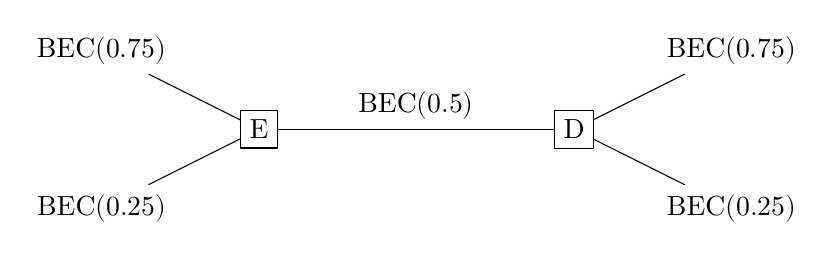
\begin{tikzpicture} [o2/.style={only=<2>}]
        \draw
            (-4, 1) node (E1) [o2] {BEC$(0.75)$}
            (-4, -1) node (E2) [o2] {BEC$(0.25)$}
            (-2, 0) node (E) [draw] {E}
            (2, 0) node (D) [draw] {D}
            (4, 1) node (D1) [o2] {BEC$(0.75)$}
            (4, -1) node (D2) [o2] {BEC$(0.25)$}
            (E1) edge [o2] (E)
            (E2) edge [o2] (E)
            (E) -- node [above] {BEC$(0.5)$} (D)
            (D) edge [o2] (D1)
            (D) edge [o2] (D2)
        ;
    \end{tikzpicture}

    \vskip1cm

    \fontsize{20pt}{20pt}\selectfont
    Suppose there are magic devices
    \tikz \node [draw] {E};
    and
    \tikz \node [draw] {D};
    that turns BEC$(x)$ into BEC$(x^2)$ and BEC$(2x - x^2)$.
\end{frame}

\begin{frame}
    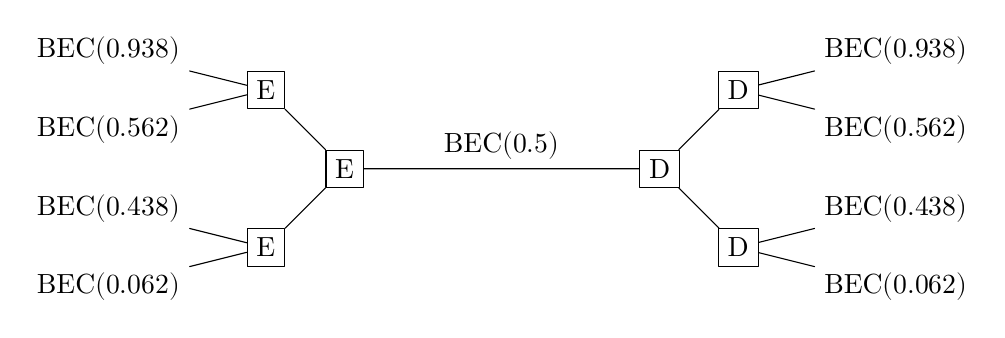
\begin{tikzpicture}
        \draw
            (-5, 1.5) node (E3) {BEC$(0.938)$}
            (-5, 0.5) node (E4) {BEC$(0.562)$}
            (-5, -0.5) node (E5) {BEC$(0.438)$}
            (-5, -1.5) node (E6) {BEC$(0.062)$}
            (-3, 1) node [draw] (E1) {E}
            (-3, -1) node [draw] (E2) {E}
            (-2, 0) node (E) [draw] {E}
            (2, 0) node (D) [draw] {D}
            (3, 1) node [draw] (D1) {D}
            (3, -1) node [draw] (D2) {D}
            (5, 1.5) node (D3) {BEC$(0.938)$}
            (5, 0.5) node (D4) {BEC$(0.562)$}
            (5, -0.5) node (D5) {BEC$(0.438)$}
            (5, -1.5) node (D6) {BEC$(0.062)$}
            (E3) -- (E1)
            (E4) -- (E1)
            (E5) -- (E2)
            (E6) -- (E2)
            (E1) -- (E)
            (E2) -- (E)
            (E) -- node [above] {BEC$(0.5)$} (D)
            (D) -- (D1)
            (D) -- (D2)
            (D1) -- (D3)
            (D1) -- (D4)
            (D2) -- (D5)
            (D2) -- (D6)
        ;
    \end{tikzpicture}

    \vskip2cm

    \fontsize{20pt}{20pt}\selectfont
    What if we apply apply more magic devices?
\end{frame}

\begin{frame}
    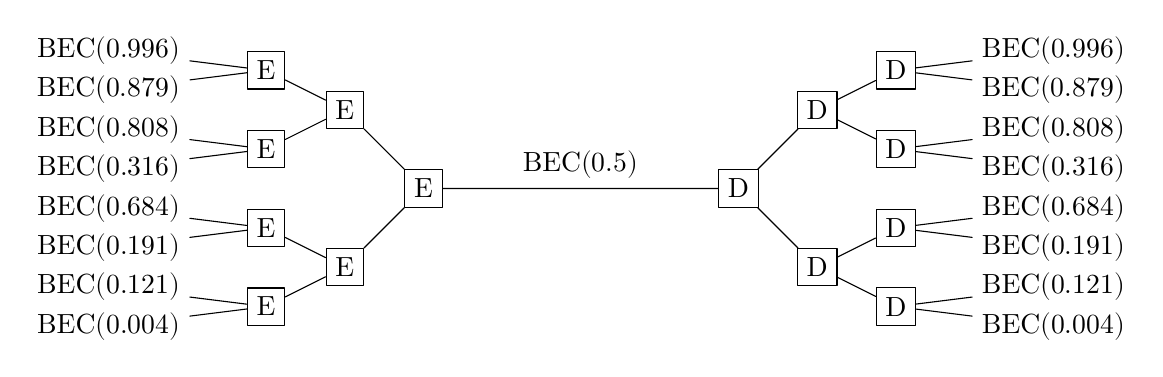
\begin{tikzpicture}
        \draw
            (-6, 1.75) node (E7) {BEC$(0.996)$}
            (-6, 1.25) node (E8) {BEC$(0.879)$}
            (-6, .75) node (E9) {BEC$(0.808)$}
            (-6, .25) node (E10) {BEC$(0.316)$}
            (-6, -.25) node (E11) {BEC$(0.684)$}
            (-6, -.75) node (E12) {BEC$(0.191)$}
            (-6, -1.25) node (E13) {BEC$(0.121)$}
            (-6, -1.75) node (E14) {BEC$(0.004)$}
            (-4, 1.5) node [draw] (E3) {E}
            (-4, 0.5) node [draw] (E4) {E}
            (-4, -0.5) node [draw] (E5) {E}
            (-4, -1.5) node [draw] (E6) {E}
            (-3, 1) node [draw] (E1) {E}
            (-3, -1) node [draw] (E2) {E}
            (-2, 0) node (E) [draw] {E}
            (2, 0) node (D) [draw] {D}
            (3, 1) node [draw] (D1) {D}
            (3, -1) node [draw] (D2) {D}
            (4, 1.5) node [draw] (D3) {D}
            (4, 0.5) node [draw] (D4) {D}
            (4, -0.5) node [draw] (D5) {D}
            (4, -1.5) node [draw] (D6) {D}
            (6, 1.75) node (D7) {BEC$(0.996)$}
            (6, 1.25) node (D8) {BEC$(0.879)$}
            (6, .75) node (D9) {BEC$(0.808)$}
            (6, .25) node (D10) {BEC$(0.316)$}
            (6, -.25) node (D11) {BEC$(0.684)$}
            (6, -.75) node (D12) {BEC$(0.191)$}
            (6, -1.25) node (D13) {BEC$(0.121)$}
            (6, -1.75) node (D14) {BEC$(0.004)$}
            (E7) -- (E3)
            (E8) -- (E3)
            (E9) -- (E4)
            (E10) -- (E4)
            (E11) -- (E5)
            (E12) -- (E5)
            (E13) -- (E6)
            (E14) -- (E6)
            (E3) -- (E1)
            (E4) -- (E1)
            (E5) -- (E2)
            (E6) -- (E2)
            (E1) -- (E)
            (E2) -- (E)
            (E) -- node [above] {BEC$(0.5)$} (D)
            (D) -- (D1)
            (D) -- (D2)
            (D1) -- (D3) 
            (D1) -- (D4)
            (D2) -- (D5)
            (D2) -- (D6)
            (D3) -- (D7)
            (D3) -- (D8)
            (D4) -- (D9)
            (D4) -- (D10)
            (D5) -- (D11)
            (D5) -- (D12)
            (D6) -- (D13)
            (D6) -- (D14)
        ;
    \end{tikzpicture}

    \vskip1.5cm

    \fontsize{20pt}{20pt}\selectfont
    What if we apply apply more magic devices? \\
    And more and more and more???
\end{frame}

\begin{frame}
    \begin{tikzpicture}
        \tikzset{
            m1/.style={alt=<3->{alerted text.fg, fill, text=white}{}},
            m2/.style={alt=<4->{alerted text.fg, fill, text=white}{}},
            m3/.style={alt=<5->{alerted text.fg, fill, text=white}{}},
            m4/.style={alt=<6->{alerted text.fg, fill, text=white}{}},
        }
        \draw
            (0, 0) node (D) [m1] {BEC$(0.5)$}
            (3, 1) node (D1) {BEC$(0.75)$}
            (3, -1) node (D2) [m2] {BEC$(0.25)$}
            (6, 1.5) node (D3) {BEC$(0.938)$}
            (6, 0.5) node (D4) {BEC$(0.562)$}
            (6, -0.5) node (D5) {BEC$(0.438)$}
            (6, -1.5) node (D6) [m3] {BEC$(0.062)$}
            (9, 1.75) node (D7) {BEC$(0.996)$}
            (9, 1.25) node (D8) {BEC$(0.879)$}
            (9, .75) node (D9) {BEC$(0.808)$}
            (9, .25) node (D10) {BEC$(0.316)$}
            (9, -.25) node (D11) {BEC$(0.684)$}
            (9, -.75) node (D12) {BEC$(0.191)$}
            (9, -1.25) node (D13) [m4] {BEC$(0.121)$}
            (9, -1.75) node (D14) {BEC$(0.004)$}
            (D) edge (D1)
            (D) edge [m2] (D2)
            (D1) edge (D3)
            (D1) edge (D4)
            (D2) edge (D5)
            (D2) edge [m3] (D6)
            (D3) edge (D7)
            (D3) edge (D8)
            (D4) edge (D9)
            (D4) edge (D10)
            (D5) edge (D11)
            (D5) edge (D12)
            (D6) edge [m4] (D13)
            (D6) edge (D14)
        ;
    \end{tikzpicture}

    \fontsize{24pt}{0}\selectfont
    \only<1>{
        \vspace*{0.5cm}
        
        This is a tree

        \vspace*{3.3cm}
    }
    \only<2->{
        \vskip-0.5cm
        \tikz [baseline=-.5ex]
        \node {\includegraphics[height=2cm]{arikan.jpg}};
        \only<-6>{E. Arıkan: This is a martingale}
        \only<7>{:Study martingale to study code}
        \vskip-0.5cm
        \[
            M_{n+1} \coloneqq
            \begin{cases*}
                2M_n - M_n^2 & with prob. $1/2$, \\
                M_n^2        & with prob. $1/2$.
            \end{cases*}
        \]
    }
\end{frame}

\begin{frame}
    \fontsize{24pt}{36pt}\selectfont
    Martingale--Code Rate Thm
    [\includegraphics[height=1cm]{arikan.jpg}]

    \pause
    \vskip2cm

    $\mathrm{Prob} \{4^{-n} < M_n < 1 - 4^{-n}\} < \varepsilon$ \\
    implies code rate \\
    $(1/2 - \varepsilon) N$ bits / $N$ channel uses.
\end{frame}

\def\murange#1#2{\tikz[x=8cm]{
	\draw [lightgray] (0, 0) -- (1/2, 0);
	\draw [Parenthesis-Parenthesis] (#1, 0) -- (#2, 0);
}}
\def\mupoint#1{\tikz[x=8cm]{
	\draw [lightgray] (0, 0) -- (1/2, 0);
	\fill (#1, 0) circle [radius=.2em];
}}
\def\WW{\includegraphics[height=1cm]{head.jpg}}

\begin{frame}
    \fontsize{16pt}{28pt}\selectfont
    $(1/2 - N^{\alert{-\rho}}) N$ bits / $N$ channel uses

    \raggedleft
    \rightskip1cm
    History of \alert{$\rho$} over BMS Channels:
                                        \hbox to4cm{$0$ \hfill $1/2$} \\
    \pause
    2015 Guruswami--Xia                              \murange{0}{1/2} \\
    2012 Goli--Hassani--Urbanke                  \murange{0}{1/3.553} \\
    2014 Hassani--Alishahi--Urbanke            \murange{1/6}{1/3.579} \\
    2014 Goldin--Burshtein                 \murange{1/5.702}{1/3.579} \\
    2016 Mondelli--Hassani--Urbanke        \murange{1/4.714}{1/3.579} \\
    2022 \WW--Lin--Vardy--Gabrys            \murange{1/4.63}{1/3.579} \\
\end{frame}

\begin{frame}
    \fontsize{12pt}{24pt}\selectfont
    \raggedleft
    \rightskip1cm
    Improve \alert{$\rho$} over BEC:    \hbox to4cm{$0$ \hfill $1/2$} \\
    \pause
    2010 Hassani--Alishahi--Urbanke
                              $2 \times 2$ \murange{1/3.589}{1/3.627} \\
    2010 Korada--Montanari--Telatar--Urbanke
                                       $2 \times 2$ \mupoint{1/3.627} \\
    2014 Fazeli--Vardy                 $8 \times 8$ \mupoint{1/3.577} \\
    2021 Trofimiuk--Trifonov         $16 \times 16$ \mupoint{1/3.346} \\
    2022 Duursma--Gabrys--Guruswami--Lin--\WW\
                                 $2 \times 2 / F_4$ \mupoint{1/3.328} \\
    2021 Trofimiuk                   $24 \times 24$ \mupoint{1/3.308} \\
    2021 Yao--Fazeli--Vardy          $32 \times 32$ \mupoint{1/3.122} \\
    2021 Yao--Fazeli--Vardy           $64 \times 64$ \mupoint{1/2.87} \\
\end{frame}

\begin{frame}
    \fontsize{16pt}{16pt}\selectfont
    \raggedleft
    \rightskip1cm
    The optimal \alert{$\rho$}:         \hbox to4cm{$0$ \hfill $1/2$} \\
                                                                  $ $ \\
    \pause
	2019 Pfister--Urbanke                               \mupoint{1/2} \\
    $q$-ary erasure channel, $q → ∞$                    \hbox to4cm{} \\
                                                                  $ $ \\
	2021 Fazeli--Hassani--Mondelli--Vardy               \mupoint{1/2} \\
    binary erasure channel                              \hbox to4cm{} \\
                                                                  $ $ \\
	2022 Guruswami--Riazanov--Ye                        \mupoint{1/2} \\
    binary symmetric memoryless channel                 \hbox to4cm{} \\
                                                                  $ $ \\
	2021 \WW--Duursma                                   \mupoint{1/2} \\
    discrete memoryless channel                         \hbox to4cm{} \\
\end{frame}

\begin{frame}
    \fontsize{16pt}{16pt}\selectfont
	2011 Alamdar-Yazdi--Kschischang: \\
	Prune the tree to reduce complexity.

    \vskip0.5cm
    
	2017 El-Khamy--Mahdavifar--Feygin--Lee--Kang: \\
    Pruning reduces complexity by a scalar; 
	still $O(N \log N)$.
    
    \vskip0.5cm

	2021 \WW--Duursma:
	$O(N \log \log N)$ \\
	Trade-off: complexity
    $\approx O(N\log(-\log(\text{decode error})))$.

    \vskip0.5cm

	2021 Mondelli--Hashemi--Cioffi--Goldsmith, \\
	2021 Hashemi--Mondelli--Fazeli--Vardy--Cioffi--Goldsmith: \\
    Study parallelism vs latency.
\end{frame}

\begin{frame}
    \fontsize{32pt}{0}\selectfont
    
    Polar code is a mathy code
    
    \pause
    \vfill
    
    \fontsize{28pt}{0}\selectfont
    Polar achieves the capacity of
\end{frame}

\begin{frame}
    \ifforloop
        \def\n{100}
    \else
        \def\n{10}
    \fi
    \begin{tikzpicture} [overlay, shift={(-4, -4)}, line width=2pt]
        \draw [magenta] plot [domain=-4:4, samples=\n]
            ({(1 + exp(\x - 3)) * sin(\x*50 + 0)},{\x});
        \draw [red] plot [domain=-4:4, samples=\n]
            ({(1 + exp(\x - 3)) * sin(\x*50 + 60)},{\x});
        \draw [yellow] plot [domain=-4:4, samples=\n]
            ({(1 + exp(\x - 3)) * sin(\x*50 + 120)},{\x});
        \draw [green] plot [domain=-4:4, samples=\n]
            ({(1 + exp(\x - 3)) * sin(\x*50 + 180)},{\x});
        \draw [cyan] plot [domain=-4:4, samples=\n]
            ({(1 + exp(\x - 3)) * sin(\x*50 + 240)},{\x});
        \draw [blue] plot [domain=-4:4, samples=\n]
            ({(1 + exp(\x - 3)) * sin(\x*50 + 300)},{\x});
    \end{tikzpicture}

    \leftskip7cm
    \fontsize{16pt}{0}\selectfont
    \parskip0pt plus1fill

	Asymmetric channel

	Multiple access channel

    Lossless compression

	Lossy compression

	Slepian--Wolf

	Lossless compression w/ helper

	Wiretap channel (degradation)
\end{frame}

\begin{frame}
    \ifforloop
        \def\n{100}
    \else
        \def\n{10}
    \fi
    \begin{tikzpicture} [overlay, shift={(6, -4)}, line width=1pt]
        \draw [magenta] plot [domain=-4:4, samples=\n]
            ({(1 + exp(\x - 3)) * sin(\x*50 + 0)},{\x});
        \draw [red] plot [domain=-4:4, samples=\n]
            ({(1 + exp(\x - 3)) * sin(\x*50 + 60)},{\x});
        \draw [yellow] plot [domain=-4:4, samples=\n]
            ({(1 + exp(\x - 3)) * sin(\x*50 + 120)},{\x});
        \draw [green] plot [domain=-4:4, samples=\n]
            ({(1 + exp(\x - 3)) * sin(\x*50 + 180)},{\x});
        \draw [cyan] plot [domain=-4:4, samples=\n]
            ({(1 + exp(\x - 3)) * sin(\x*50 + 240)},{\x});
        \draw [blue] plot [domain=-4:4, samples=\n]
            ({(1 + exp(\x - 3)) * sin(\x*50 + 300)},{\x});
    \end{tikzpicture}

    \leftskip0cm
    \fontsize{16pt}{0}\selectfont
    \parskip0pt plus1fill
    
    Deletion channel ... (good error prob)
    
    Broadcast channel ... (good error prob)

    Channel with memory ... (good error prob)

    Wiretap channel (no degradation) ... (good error prob)

    Hidden Markov chain channel state ... (good error prob)

    Non-stationary channel ... (good gap to capacity)

    Classical--Quantum channel ... (yes)

    Quantum--Quantum channel ... (?)
\end{frame}

\begin{frame}
    \includegraphics[height=4cm]{sudoku.png}\llap{\tiny Wikipedia}

    \vskip0.5cm

    \fontsize{36pt}{36pt}\selectfont
    Low-Density Parity-Check (LDPC) Codes
\end{frame}

\begin{frame}
    \fontsize{36pt}{36pt}\selectfont
    Rule: Every
    \fontsize{18pt}{0}\selectfont
    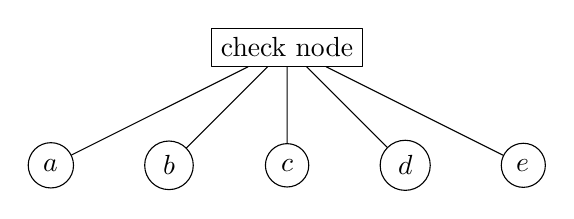
\begin{tikzpicture}[x=1.5cm, y=1.5cm]
        \draw
            (0, 1) node (C) [draw] {check node}
            (-2, 0) node (V) [draw, circle] {$a$} (V) -- (C)
            (-1, 0) node (V) [draw, circle] {$b$} (V) -- (C)
            (0, 0) node (V) [draw, circle] {$c$} (V) -- (C)
            (1, 0) node (V) [draw, circle] {$d$} (V) -- (C)
            (2, 0) node (V) [draw, circle] {$e$} (V) -- (C)
        ;
    \end{tikzpicture}

    \fontsize{36pt}{36pt}\selectfont
    Sum to an even number

    \vskip1cm
    \pause

    \fontsize{12pt}{0}\selectfont
    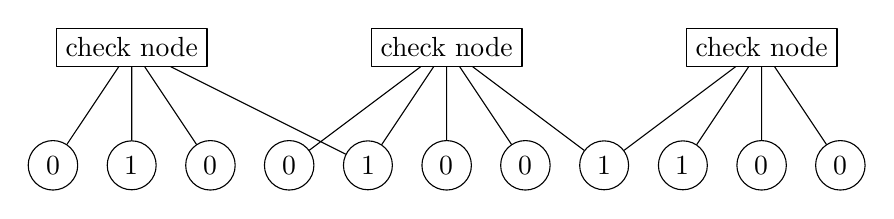
\begin{tikzpicture}[y=1.5cm]
        \draw
            (-4, 1) node (A) [draw] {check node}
            (0, 1) node (B) [draw] {check node}
            (4, 1) node (C) [draw] {check node}
            (-5, 0) node (V) [draw, circle] {$0$} (V) -- (A)
            (-4, 0) node (V) [draw, circle] {$1$} (V) -- (A)
            (-3, 0) node (V) [draw, circle] {$0$} (V) -- (A)
            (-2, 0) node (V) [draw, circle] {$0$} (V) -- (B)
            (-1, 0) node (V) [draw, circle] {$1$} (V) -- (B) (V) -- (A)
            (0, 0) node (V) [draw, circle] {$0$} (V) -- (B)
            (1, 0) node (V) [draw, circle] {$0$} (V) -- (B)
            (2, 0) node (V) [draw, circle] {$1$} (V) -- (B) (V) -- (C)
            (3, 0) node (V) [draw, circle] {$1$} (V) -- (C)
            (4, 0) node (V) [draw, circle] {$0$} (V) -- (C)
            (5, 0) node (V) [draw, circle] {$0$} (V) -- (C)
        ;
    \end{tikzpicture}
\end{frame}

\def\erase{\includegraphics[height=1cm]{head}}

\begin{frame}
    \begin{tikzpicture}
        \tikzset{
            a1/.style={alt=<2>{alerted text.fg}{}},
            a2/.style={alt=<3>{alerted text.fg}{}},
            a3/.style={alt=<4>{alerted text.fg}{}},
            o1/.style={a1, only=<2->},
            o2/.style={a2, only=<3->},
            o3/.style={a3, only=<4->},
        }
        \draw
            (-3, 2) node (A) [draw, a1] {check node}
            (0, 2) node (B) [draw, a2] {check node}
            (4, 2) node (C) [draw, a3] {check node}
            (-5, 0) node (V) [draw, circle] {$0$} (V) edge [a1] (A)
            (-4, 0) node (V) [draw, circle] {$1$} (V) edge [a1] (A)
            (-3, 0) node (V) [draw, circle] {$0$} (V) edge [a1] (A)
            (-2, 0) node (V) [draw, circle] {$0$} (V) edge [a2] (B)
            (-1, 0) node (V) {\erase}             (V) edge [a2] (B)
                                                  (V) edge [a1] (A)
            (-1, -1) node [draw, circle, o1] {1}
            (0, 0) node (V) [draw, circle] {$0$} (V) edge [a2] (B)
            (1, 0) node (V) [draw, circle] {$0$} (V) edge [a2] (B)
            (2, 0) node (V) {\erase}             (V) edge [a2] (B)
                                                 (V) edge [a3] (C)
            (2, -1) node [o1] {\erase}
            (2, -2) node [draw, circle, o2] {1}
            (3, 0) node (V) [draw, circle] {$1$} (V) edge [a3] (C)
            (4, 0) node (V) [draw, circle] {$0$} (V) edge [a3] (C)
            (5, 0) node (V) {\erase}             (V) edge [a3] (C)
            (5, -1) node [o1] {\erase}
            (5, -2) node [o2] {\erase}
            (5, -3) node [draw, circle, o3] {0}
            (-1, -4.5) node [only=<5->, alerted text.fg]
                {\fontsize{16pt}{0}\selectfont
                How to analyze, mathematically?}
        ;
    \end{tikzpicture}
\end{frame}

\begin{frame}
    \begin{tikzpicture}
        \draw
            (-3, 2) node (A) [draw] {check node}
            [every node/.style={rotate=-60}]
            (-5, 0) node (V) {BEC$(a)$} (V) -- (A)
            (-4, 0) node (V) {BEC$(b)$} (V) -- (A)
            (-3, 0) node (V) {BEC$(c)$} (V) -- (A)
            (-1, 0) node (V) {BEC$(x)$} (V) -- (A)
            (5.5, 0)
        ;
        \node at (-2, 0.5) 
            [only=<2->, alerted text.fg, right, rotate=-60]
            {BEC$(x - x(1-a)(1-b)(1-c))$}
        ;
    \end{tikzpicture}
\end{frame}

\begin{frame}
    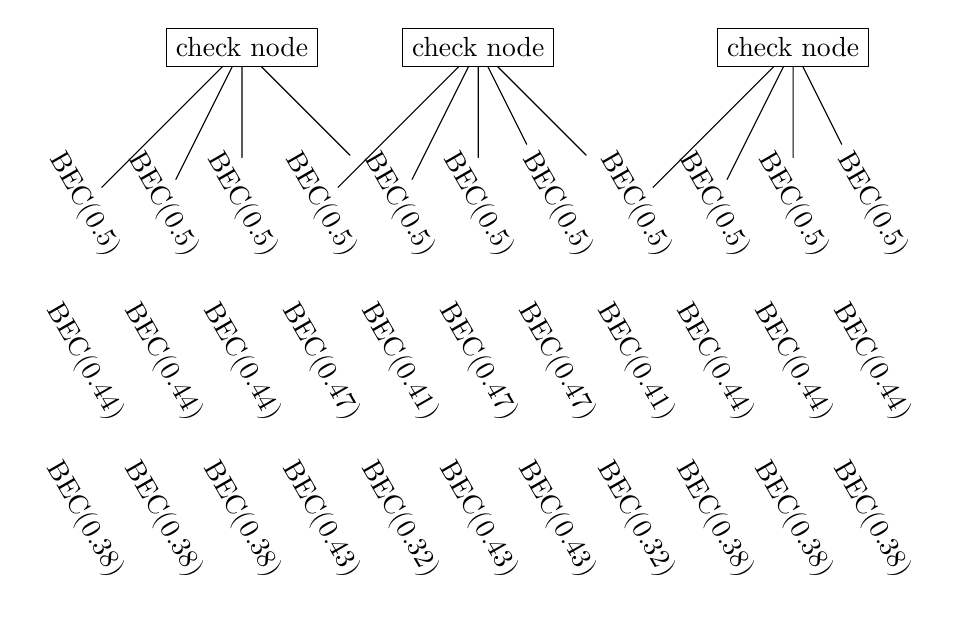
\begin{tikzpicture}
        \draw
            (-3, 2) node (A) [draw] {check node}
            (0, 2) node (B) [draw] {check node}
            (4, 2) node (C) [draw] {check node}
            [every node/.style={rotate=-60}]
            (-5, 0) node (V) {BEC$(0.5)$} (V) -- (A)
            (-4, 0) node (V) {BEC$(0.5)$} (V) -- (A)
            (-3, 0) node (V) {BEC$(0.5)$} (V) -- (A)
            (-2, 0) node (V) {BEC$(0.5)$} (V) -- (B)
            (-1, 0) node (V) {BEC$(0.5)$} (V) -- (B)
                                          (V) -- (A)
            (0, 0) node (V) {BEC$(0.5)$} (V) -- (B)
            (1, 0) node (V) {BEC$(0.5)$} (V) -- (B)
            (2, 0) node (V) {BEC$(0.5)$} (V) -- (B)
                                         (V) -- (C)
            (3, 0) node (V) {BEC$(0.5)$} (V) -- (C)
            (4, 0) node (V) {BEC$(0.5)$} (V) -- (C)
            (5, 0) node (V) {BEC$(0.5)$} (V) -- (C)
        ;
        \draw [only=<2->, every node/.style={rotate=-60}]
            (-5, -2) node {BEC$(0.44)$}
            (-4, -2) node {BEC$(0.44)$}
            (-3, -2) node {BEC$(0.44)$}
            (-2, -2) node {BEC$(0.47)$}
            (-1, -2) node {BEC$(0.41)$}
            (0, -2) node {BEC$(0.47)$}
            (1, -2) node {BEC$(0.47)$}
            (2, -2) node {BEC$(0.41)$}
            (3, -2) node {BEC$(0.44)$}
            (4, -2) node {BEC$(0.44)$}
            (5, -2) node {BEC$(0.44)$}
        ;
        \draw [only=<3->, every node/.style={rotate=-60}]
            (-5, -4) node {BEC$(0.38)$}
            (-4, -4) node {BEC$(0.38)$}
            (-3, -4) node {BEC$(0.38)$}
            (-2, -4) node {BEC$(0.43)$}
            (-1, -4) node {BEC$(0.32)$}
            (0, -4) node {BEC$(0.43)$}
            (1, -4) node {BEC$(0.43)$}
            (2, -4) node {BEC$(0.32)$}
            (3, -4) node {BEC$(0.38)$}
            (4, -4) node {BEC$(0.38)$}
            (5, -4) node {BEC$(0.38)$}
        ;
    \end{tikzpicture}
\end{frame}

\begin{frame}
    \uncover<1->{\includegraphics[height=4cm]{ice1.jpg}}
    \uncover<2->{\includegraphics[height=4cm]{ice2.jpg}}
    \uncover<3->{\includegraphics[height=4cm]{ice3.jpg}}
    \uncover<4->{\includegraphics[height=4cm]{ice4.jpg}}
\end{frame}

\begin{frame}
    \fontsize{32pt}{0}\selectfont
    
    LDPC code is a physics code
    
    \pause
    \vfill
    
    \fontsize{28pt}{0}\selectfont
    Works well but hard to analyze
\end{frame}

\def\KTV#1{\relax%
    \pdfliteral{q 1 J 1 j 1 Tr}%
    \color{white}%
    \pgfsetlinewidth{2pt}%
    \rlap{#1}%
    \pdfliteral{Q}%
    #1%
}

\begin{frame}
    \begin{tikzpicture}[overlay]
        \fontsize{36pt}{0}\selectfont
        \draw
            node {\includegraphics[height=8.5cm]{zeus.jpg}}
            (4.5, 4) node {\tiny Wikipedia}
            (1, 3.5) node {\KTV{Society}}
            (-2, 0.5) node {\KTV{LDPC}}
            (2, -1) node {\KTV{Polar}}
            (-4, -1) node [scale=0.5] {\KTV{Turbo}}
            (-2, -2) node [scale=0.5] {\KTV{Reed--Muller}}
            (0, -3.5) node {\KTV{Channel Evolution}}
        ;
    \end{tikzpicture}
\end{frame}

\begin{frame}
    \begin{tikzpicture} [overlay]
        \path
            (0, -1)node {\includegraphics[height=11cm]{radagon.jpeg}}
            (0, -1) node [white]
            {\fontsize{32pt}{0}\selectfont Challenges}
            (3, 4) node {\tiny Game: Elden Ring}
        ;
    \end{tikzpicture}
\end{frame}

\def\sun#1#2{
    \ifforloop
        \def\n{200}
    \else
        \def\n{10}
    \fi
    \path [overlay]
        foreach \r in {1, ..., \n}{
            (
                {Mod(13.75 * \r, 36) * 10}
                :
                {sqrt(\r)} * 0.6
            )
            node [scale=200/(100+\r)] {\emoji{#2}}
        }
        (0, 0) node [scale=10] {\emoji{#1}}
    ;
}

\begin{frame}
    \begin{tikzpicture}
        \only<1>{\sun{tokyo-tower}{mobile-phone}}
        \only<2>{\sun{hospital}{mask}}
        \only<3>{\sun{mag}{scroll}}
    \end{tikzpicture}
\end{frame}

\begin{frame}
    \fontsize{9pt}{16pt}\selectfont
    \begin{tabular}{cccc}
        \toprule
        Problem & There are $n$ & $k$ of them & To solve, use $m$\\
        \midrule
        Radio protocol & cellphones & want to talk & frequencies \\
        Disease control & people & are sick & virus tests \\
        Search engine
        & webpages & contain keywords & bits per keyword \\
        \midrule
        \uncover<2>{Radio protocol & messages & will be sent & frequencies} \\
        \uncover<2>{Genotyping & genes & cause cancer & gene tests} \\
        \uncover<2>{Computer forensics & files & will be modified & bits of storage} \\
        \uncover<2>{Property-preserving hash & properties & appears in a file & bits per file} \\
        \uncover<2>{Image compression & wavelet coefficients & are nonzero & bits per digit} \\
        \uncover<2>{Traitor tracing & users & resell keys & keys} \\
        \uncover<2>{Heavy hitter / DoS & users & are spamming  & virtual servers} \\
        \bottomrule
    \end{tabular}
\end{frame}

\def\sun[#1]#2{
    \path [#1]
        foreach \r in {1, ..., #2}{
            (
                {Mod(13.75 * \r, 36) * 10}
                :
                {sqrt(\r)} * 0.4
            )
            node [scale=150/(100+\r)] {\emoji{mobile-phone}}
        }
        (0, 0) node [scale=3] {\emoji{tokyo-tower}}
    ;
}

\begin{frame}
    \fontsize{24pt}{36pt}\selectfont
    Proposal: Prove the following

    \vskip2cm

    \fontsize{12}{0}\selectfont
    \begin{tikzpicture}
        \sun[overlay, shift={(-4, 0)}]{20}
        \node [scale=5] {\emoji{right-arrow}} ;
        \sun[overlay, shift={(4, 2)}]{10}
        \sun[overlay, shift={(4, -2)}]{10}
    \end{tikzpicture}

    \vspace*{1cm}
\end{frame}

\begin{frame}
    \fontsize{24pt}{36pt}\selectfont
    Proposal: Prove the following.

    \vskip1cm

    Lemma [Your Name Here] \\
    If we can solve $(n, k)$-RAC \\
    {\fontsize{18pt}{18pt}\selectfont (RAC = random access channel), \\}
    then we can solve $(3n, 2k)$-RAC.

    \vspace*{1cm}
\end{frame}

\begin{frame}
    \begin{tikzpicture} [overlay]
        \path
            node {\includegraphics[height=10cm]{elden.jpeg}}
            (-1, -2.5) node [white, rotate=-12]
            {\fontsize{32pt}{0}\selectfont CHALLENGES}
            (6.5, 4) node {\tiny Game: Elden Ring}
        ;
    \end{tikzpicture}
\end{frame}

\begin{frame}
    \begin{tikzpicture}
        \draw
            (0, 6)
            (2, 6) node[overlay]{\includegraphics[height=15cm]{dna.pdf}}
            (12, 7.5) node {\fontsize{18pt}{0}\selectfont DNA Coding}
            (11, 6) node [right] {Substitution}
            (11, 5) node [right] {Insertion}
            (11, 4) node [right] {Deletion}
            (11, 3) node [right] {Transposition}
            (11, 2) node [right] {Amplification}
            (11, 1) node [right] {Permutation}
        ;
    \end{tikzpicture}
\end{frame}

\begin{frame}
    \begin{tikzpicture}
        \draw [a/.style={alerted text.fg, shift={(-1, 0)}}]
            (0, 6) node [overlay, xshift=-2.9cm]
            {\includegraphics[height=15cm]{dna.pdf}}
            (12, 7.5) node {\fontsize{18pt}{0}\selectfont DNA Coding}
            (11, 6) node [right, alt=<1>{a}{}] {Substitution}
            (11, 5) node [right, alt=<2>{a}{}] {Insertion}
            (11, 4) node [right, alt=<3>{a}{}] {Deletion}
            (11, 3) node [right, alt=<4>{a}{}] {Transposition}
            (11, 2) node [right, alt=<5>{a}{}] {Amplification}
            (11, 1) node [right, alt=<6>{a}{}] {Permutation}
        ;
        \path [overlay, only=<1>, shift={(6, 6)}]
            (0, 1) node [scale=2] {ATTCCG}
            (0, 0) node [scale=2] {~\emoji{down-arrow}}
            (0, -1) node [scale=2] {ATT\alert{A}CG}
        ;
        \path [overlay, only=<2>, shift={(6, 5)}]
            (0, 0.5) node [scale=2] {ATT~~CCG}
            (0, 0) node [scale=2] {\emoji{up-arrow}~~}
            (0, -1) node [scale=2] {G~~}
        ;
        \path [overlay, only=<3>, shift={(6, 4)}]
            (0, 0) node [scale=2] {ATT~C~CG}
            (0, 0) node [scale=2] {~\emoji{cross-mark}}
        ;
        \path [overlay, only=<4>, shift={(6, 3)}]
            (0, 1) node [scale=2] {ATTCCG}
            (0,0)node[scale=2,rotate=-90]{\emoji{shuffle-tracks-button}}
            (0, -1) node [scale=2] {AT\alert{CT}CG}
        ;
        \path [overlay, only=<5>, shift={(6, 2)}]
            (-1, 0) node [scale=2] {\emoji{dna}}
            (0, 0) node [scale=2] {\emoji{right-arrow}}
            (1, 0.5) node [scale=2] {\emoji{dna}}
            (1, -0.5) node [scale=2] {\emoji{dna}}
        ;
        \path [overlay, only=<6>, shift={(6, 1)}]
            (-1, 0.5) node [scale=2] {\emoji{dna}}
            (-1, -0.5) node [scale=2] {\emoji{dna}}
            (0, 0) node [scale=2] {\emoji{shuffle-tracks-button}}
            (1, 0.5) node [scale=2] {\emoji{dna}}
            (1, -0.5) node [scale=2] {\emoji{dna}}
        ;
    \end{tikzpicture}
\end{frame}

\begin{frame}
    \begin{tikzpicture}
        \draw [a/.style={alerted text.fg, shift={(-1, 0)}}]
            (0, 6) node [overlay, xshift=-5.8cm]
            {\includegraphics[height=15cm]{dna.pdf}}
            (12, 7.5) node {\fontsize{18pt}{0}\selectfont DNA Coding}
            (11, 6) node[right,alt={<1,3,4,5,7,8,9>{a}{}}]{Substitution}
            (11, 5) node [right, alt={<2,4,9>{a}{}}] {Insertion}
            (11, 4) node [right, alt={<2,4,9>{a}{}}] {Deletion}
            (11, 3) node [right, alt={<3,4,9>{a}{}}] {Transposition}
            (11, 2) node [right, alt={<5,8,9>{a}{}}] {Amplification}
            (11, 1) node [right, alt={<6,7,8,9>{a}{}}] {Permutation}
        ;
        \path [overlay, only=<1>]
            (4, 6) node [align=center] {Traditional\\coding\\problem}
        ;
        \path [overlay, only=<2>]
            (4, 4.5) node [align=center] {Synchronization\\problem}
        ;
        \path [overlay, only=<3>]
            (4, 4.5) node [align=center] {Channels\\with\\memory}
        ;
        \path [overlay, only=<4>]
            (4, 4.5) node [align=center] {Polar code\\OK}
        ;
        \path [overlay, only=<5>]
            (4, 4) node [align=center] {Trace\\reconstruction\\problem}
        ;
        \path [overlay, only=<6>]
            (4, 1) node [align=center]
            {Use empirical\\distribution\\as codeword}
        ;
        \path [overlay, only=<7>]
            (4, 3.5) node [align=center] {Network\\coding}
        ;
        \path [overlay, only=<8>]
            (4, 3.5) node [align=center] {Clustering\\problem}
        ;
        \path [overlay, only=<9>]
            (4, 3.5) node [scale=5] {\emoji{shrug}}
        ;
    \end{tikzpicture}
\end{frame}

\bibliographystyle{unsrt}
\bibliography{ChannelManipul}

\end{document}


It looks like a promising thing to document
Recommend Arikan's tutorial